\let\negmpace\undefined
\let\negthickspace\undefined
\documentclass[journal]{IEEEtran}
\usepackage[a5paper, margin=10mm, onecolumn]{geometry}
%\usepackage{lmodern} % Ensure lmodern is loaded for pdflatex
\usepackage{tfrupee} % Include tfrupee package
\setlength{\headheight}{1cm} % Set the height of the header box
\setlength{\headsep}{0mm}     % Set the distance between the header box and the top of the text
\usepackage{xparse}
\usepackage{gvv-book}
\usepackage{gvv}
\usepackage{cite}
\usepackage{amsmath,amssymb,amsfonts,amsthm}
\usepackage{algorithmic}
\usepackage{graphicx}
\usepackage{textcomp}
\usepackage{xcolor}
\usepackage{txfonts}
\usepackage{listings}
\usepackage{enumitem}
\usepackage{mathtools}
\usepackage{gensymb}
\usepackage{comment}
\usepackage[breaklinks=true]{hyperref}
\usepackage{tkz-euclide} 
\usepackage{listings}
% \usepackage{gvv}                                        
\def\inputGnumericTable{}                                 
\usepackage[latin1]{inputenc}                                
\usepackage{color}                                            
\usepackage{array}                                            
\usepackage{longtable}                                       
\usepackage{calc}                                             
\usepackage{multirow}                                         
\usepackage{hhline}                                           
\usepackage{ifthen}                                           
\usepackage{lscape}
\usepackage{float}
\renewcommand{\thefigure}{\theenumi}
\renewcommand{\thetable}{\theenumi}
\setlength{\intextsep}{10pt} % Space between text and floats
\numberwithin{equation}{enumi}
\numberwithin{figure}{enumi}
\renewcommand{\thetable}{\theenumi}
\begin{document}
\bibliographystyle{IEEEtran}
\title{9-9.3-13}
\author{EE24BTECH11030 - J.KEDARANANDA}
% \maketitle
% \newpage
% \bigskip
{\let\newpage\relax\maketitle}
\textbf{Question}:\\
Find the area bounded by the ellipse $x^2 + 4y^2 = 16$ and the ordinates x = 0 and x = 2.
\\
\solution \\
\begin{table}[h!]    
  \centering
  \begin{tabular}[12pt]{ |c|c|}
    \hline
    \textbf{Variable} & \textbf{Description}\\ 
    \hline
    $\vec{x_1},\vec{x_2},\vec{x_3},\vec{x_4}$ &  intersection points\\
    \hline
    $\vec{h}$ & Point on the given line\\
    \hline
    $\vec{m}$ & Direction vector of given line\\
    \hline
    $A$ & Area of the region\\
    \hline
\end{tabular}

  \caption{}
  \label{tab1-9.3-13}
\end{table}\\
\begin{table}[h!]    
  \centering
  \begin{tabular}[12pt]{ |c|c|}
    \hline
    \textbf{Conic} & \textbf{expression}\\ 
    \hline
    ellipse & $\vec{x}^\top\vec{V}\vec{x} + 2\vec{u}^\top\vec{x} + f = 0$\\
    \hline
    line & $\vec{x}=\vec{h}+\kappa\vec{m}$\\
    \hline
\end{tabular}

  \caption{}
  \label{tab2-9.3-13}
\end{table}\\
\begin{align}
\vec{V}&=\myvec{\frac{1}{16} & 0\\0 & \frac{1}{4}}\\
\vec{u}&=\myvec{0\\0}\\
f&=-1
\end{align}
For the given line $x=2$, The values of $\vec{h}$, $\vec{m}$ are
\begin{align}
\vec{h}&=\myvec{0\\0}\\
\vec{m}&=\myvec{1\\0}
\end{align}
From \ref{tab1-9.3-13} and \ref{tab2-9.3-13} , The intersection points are
\begin{align}
\vec{x_1} &= \myvec{2\\\sqrt{3}}\\
\vec{x_2} &= \myvec{2\\-\sqrt{3}}\\
\vec{x_3} &= \myvec{0\\2}\\
\vec{x_4} &= \myvec{0\\-2}\\
\end{align}
\begin{align}
y &= \pm \sqrt{4 - \frac{1}{4}x^2}
\end{align}
The area A  between the curves from \( x = 0 \) to \( x = 2 \) is given by:
\begin{align}
A = 4 \int_0^2 \sqrt{1 - \frac{x^2}{16}} \, dx
\end{align}
So by simplyfing :
\begin{align}
A = 2\sqrt{3} + \frac{4\pi}{3}
\end{align}

\begin{figure}[!ht]
    \centering
    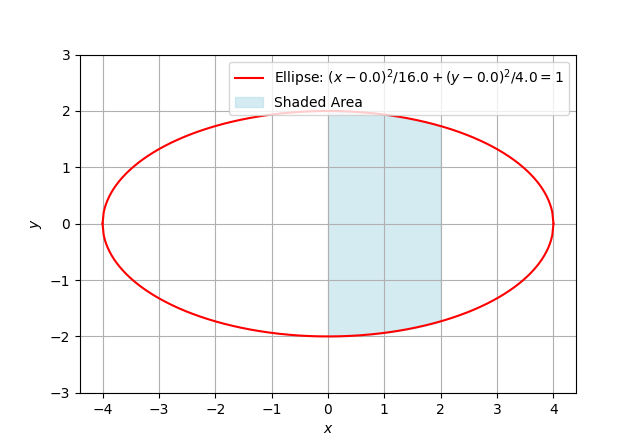
\includegraphics[width=\linewidth]{figs/fig1.png}
    \caption{}
\end{figure}
\end{document}
